% !TEX program = xelatex
\documentclass[a4paper,11pt]{article}
\usepackage{graphicx} % Required for inserting images
\usepackage[]{geometry} % Insert size in the [] to define and control the margins on the page
\usepackage{hyperref} % Makes links and table of contents clickable
% \hypersetup{colorlinks=true, linkcolor=blue} Use this if you want the links to be noticeable and have color blue, the color can be changed
% \usepackage{mathtools} % math tools builds upon amsmath, so only one of them is needed, note that mathtools has all the functions that amsmath has and even more
\usepackage{amsmath ,amssymb,amsthm}
\usepackage{tikz}
\usepackage{tikz-cd}
\renewcommand{\qed}{\hfill\blacksquare}
\newcommand{\D}[1]{\Delta #1}
\renewcommand{\a}{\alpha}
% \newcommand{\a}{\alpha}
\usepackage{cancel}
\usepackage{float}
% ============================================================ %

% HEBREW support via polyglossia %

% ============================================================ %

\usepackage{polyglossia}

\defaultfontfeatures{Mapping=tex-text, Scale=MatchLowercase}

\setdefaultlanguage{hebrew}

\setotherlanguage{english}

\newfontfamily\hebrewfont[Script=Hebrew]{Arial}

% Use \begin{hebrew} block of text \end{hebrew} for paragraphs.

% Use \texthebrew{ } and \textenglish{ } for short texts.

% ============================================================ %

\usepackage{bidi} % we use bidi for Right-To-Left (RTL) writing
\title{מאקרו א' - תרגול 1}
\author{מתן לבינטוב}
\date{}
% Begin of Document ---------------------------------------- %
\begin{document}
\begin{RTL}
    
% Title ---------------------------------------- %
\maketitle
% \newpage
% Table of Contents ---------------------------------------- %
% \tableofcontents
% \newpage
% Start of paper ---------------------------------------- %
\section{הקדמה}
בתרגול הזה נדבר על מודל $IS-LM$  בטווח הקצר במשק סגור 
\section{הנחות המודל}
\begin{itemize}
    \item התוצר נקבע בטווח קצר לפי ביקוש
    \item בטווח קצר המחירים קשיחים
    \item המשק יכול בנקודת שיווי משקל אשר גבוהה יותר או נמוכה יותר מתוצר פוטנציאלי
\end{itemize}
\section{עקומת $IS$ - שוק המוצרים}
עקומת $IS$ הינה העקומה אשר על גביה נמצאים אוסף הצירופים של תוצר וריבית אשר מביעים לש''מ בשוק המוצרים
\begin{align*}
    \begin{split}
        IS : Y &= C + I + G \\
        C & = C_0 + cY^d = C_0  + c\left( Y-T \right)  ; \quad T = T_0 + tY \\
        I & =   I_0 - bi \\ 
        G &= G_0 \\ 
    \end{split}
\end{align*}

\begin{equation*}
    IS : Y = \alpha \left( A_0 - bi \right) \qquad \alpha = \frac{1}{1-c(1-t)} \: \text{המכפיל הקיינסיאני}
\end{equation*}
\begin{equation*}
    A_0 = C_0 - cT_o + I_0 + G_0
\end{equation*}

\subsection{שיפוע העקומה}
בגלל הצירים שיפוע העקומה צריך להיות לפי $\frac{\partial i}{\partial Y}$.
אולם יותר קל לגזור את העקומה שהיא לפי $\frac{\partial Y}{\partial i}$ ופשוט לעלות בחזקת מינוס 1
\begin{equation*}
    \frac{\partial Y}{\partial i} = - \alpha b \implies \frac{\partial i}{\partial Y } = \frac{-1}{\alpha b}
 \end{equation*}

\subsection{היסטים}
$\Delta Y = \alpha \left[\Delta A_0 - b\Delta i\right]$  \vspace{10pt}
\\
\textbf{היסט אופקי } $\Delta i = 0 $ \vspace{10pt} 
\\
$\D{Y} = \a \D{A_0}$ \vspace{10pt}
\\ 
\textbf{היסט אנכי } $\D{Y} = 0 $ \vspace{10pt}
\\
$\D{i} = \dfrac{\D{A_0}}{b}$
\end{RTL}
\begin{tikzpicture}[scale=2]
    \draw[->] (0,0) -- (6,0) node[right] {$Y$};
    \draw[->] (0,0) -- (0,5) node[above] {$i$};
    % \draw[dashed] (0,4) -- (4,0) node[midway, above left] {up} node[midway, below right] {down};
    \draw [blue] (0.5,3.5) -- (4.5,0.5) node[midway, above left] {};
    \node[right] at (3,3) {היצע עודף};
    \node[left] at (2.5,1) {ביקוש עודף};
    \node[right] at (4.5,0.5) {$IS$};

\end{tikzpicture}
\newpage

\begin{RTL}    
\section{עקומת $LM$ - שוק הכסף}
עקומת LM היא עקומה אשר על גביה נמצאים אוסף הצירופים של תוצר וריבית אשר מביאים לשיווי משקל
בשוק הכסף. 
\begin{align*}
    \begin{split}
       LM : \left(\frac{M}{P}\right) ^ d  & = M ^ s \\ 
       \left(\frac{M}{P}  \right) ^ d    & = M_0 + kY - hi 
    \end{split}
\end{align*}
\begin{itemize}
    \item $M_0$ הינו מינע הביטחון
    \item $k$ מניע עסקאות
    \item $h$ מניע ספקולטיבי
\end{itemize}

\begin{equation*}
    LM : i  = \frac{1}{h} \left[ky + M_0 - M^s \right]
\end{equation*}

\begin{tikzpicture}[scale=1.4]
    \draw[->] (0,0) -- (6,0) node[right] {$Y$};
    \draw[->] (0,0) -- (0,5) node[above] {$i$};
    % \draw[dashed] (0,4) -- (4,0) node[midway, above left] {up} node[midway, below right] {down};
    \draw [red] (0.5,0.5) -- (4.5,4.5) node[midway, above left] {};
    \node[right] at (1,3) {היצע עודף};
    \node[left] at (4,1) {ביקוש עודף};
    \node[right] at (4.5,4.5) {$LM$};
\end{tikzpicture}



\subsection{היסטים}

$\Delta i = \dfrac{1}{h} \left[k\D{Y} + \D{M_0} - \D{M^s}\right]$  \vspace{10pt}
\\
\textbf{היסט אופקי } $\Delta i = 0 $ \vspace{10pt} 
\\
$\D{Y} = \dfrac{\D{M^s} - \D{M_0}}{k}$ \vspace{10pt}
\\ 
\textbf{היסט אנכי } $\D{Y} = 0 $ \vspace{10pt}
\\
$\D{i} = \dfrac{\D{M_0} - \D{M^s} }{h}$

\section{שיווי משקל כללי}
קיים שילוב יחיד של תוצר וריבית אשר מביא לשיווי משקל בשוק המוצרים ובשוק הכסף במקביל לכל מצב
עולם.
שילוב של שתי העקומות הצבה של שוק הכסף בשוק המוצרים דרך הריבית.
\begin{equation*}
    Y=\frac{\alpha h}{h+\alpha b k} \times A_0+\frac{\alpha b}{h+\alpha b k} \times\left(M^s-M_0\right)
\end{equation*}
% \begin{tikzpicture}[scale=1.4]
%     \draw[->] (0,0) -- (6,0) node[right] {$Y$};
%     \draw[->] (0,0) -- (0,5) node[above] {$i$};
%     % \draw[dashed] (0,4) -- (4,0) node[midway, above left] {up} node[midway, below right] {down};
%     \draw [red] (0.5,0.5) -- (4.5,4.5) node[midway, above left] {};
%     \node[right] at (4.5,4.5) {$LM$};
%     \draw [blue] (0.5,3.5) -- (4.5,0.5) node[midway, above left] {};
%     \node[right] at (4.5,0.5) {$IS$};

% \end{tikzpicture}
\begin{figure}[H]
    % \begin{small}
        \begin{center}
            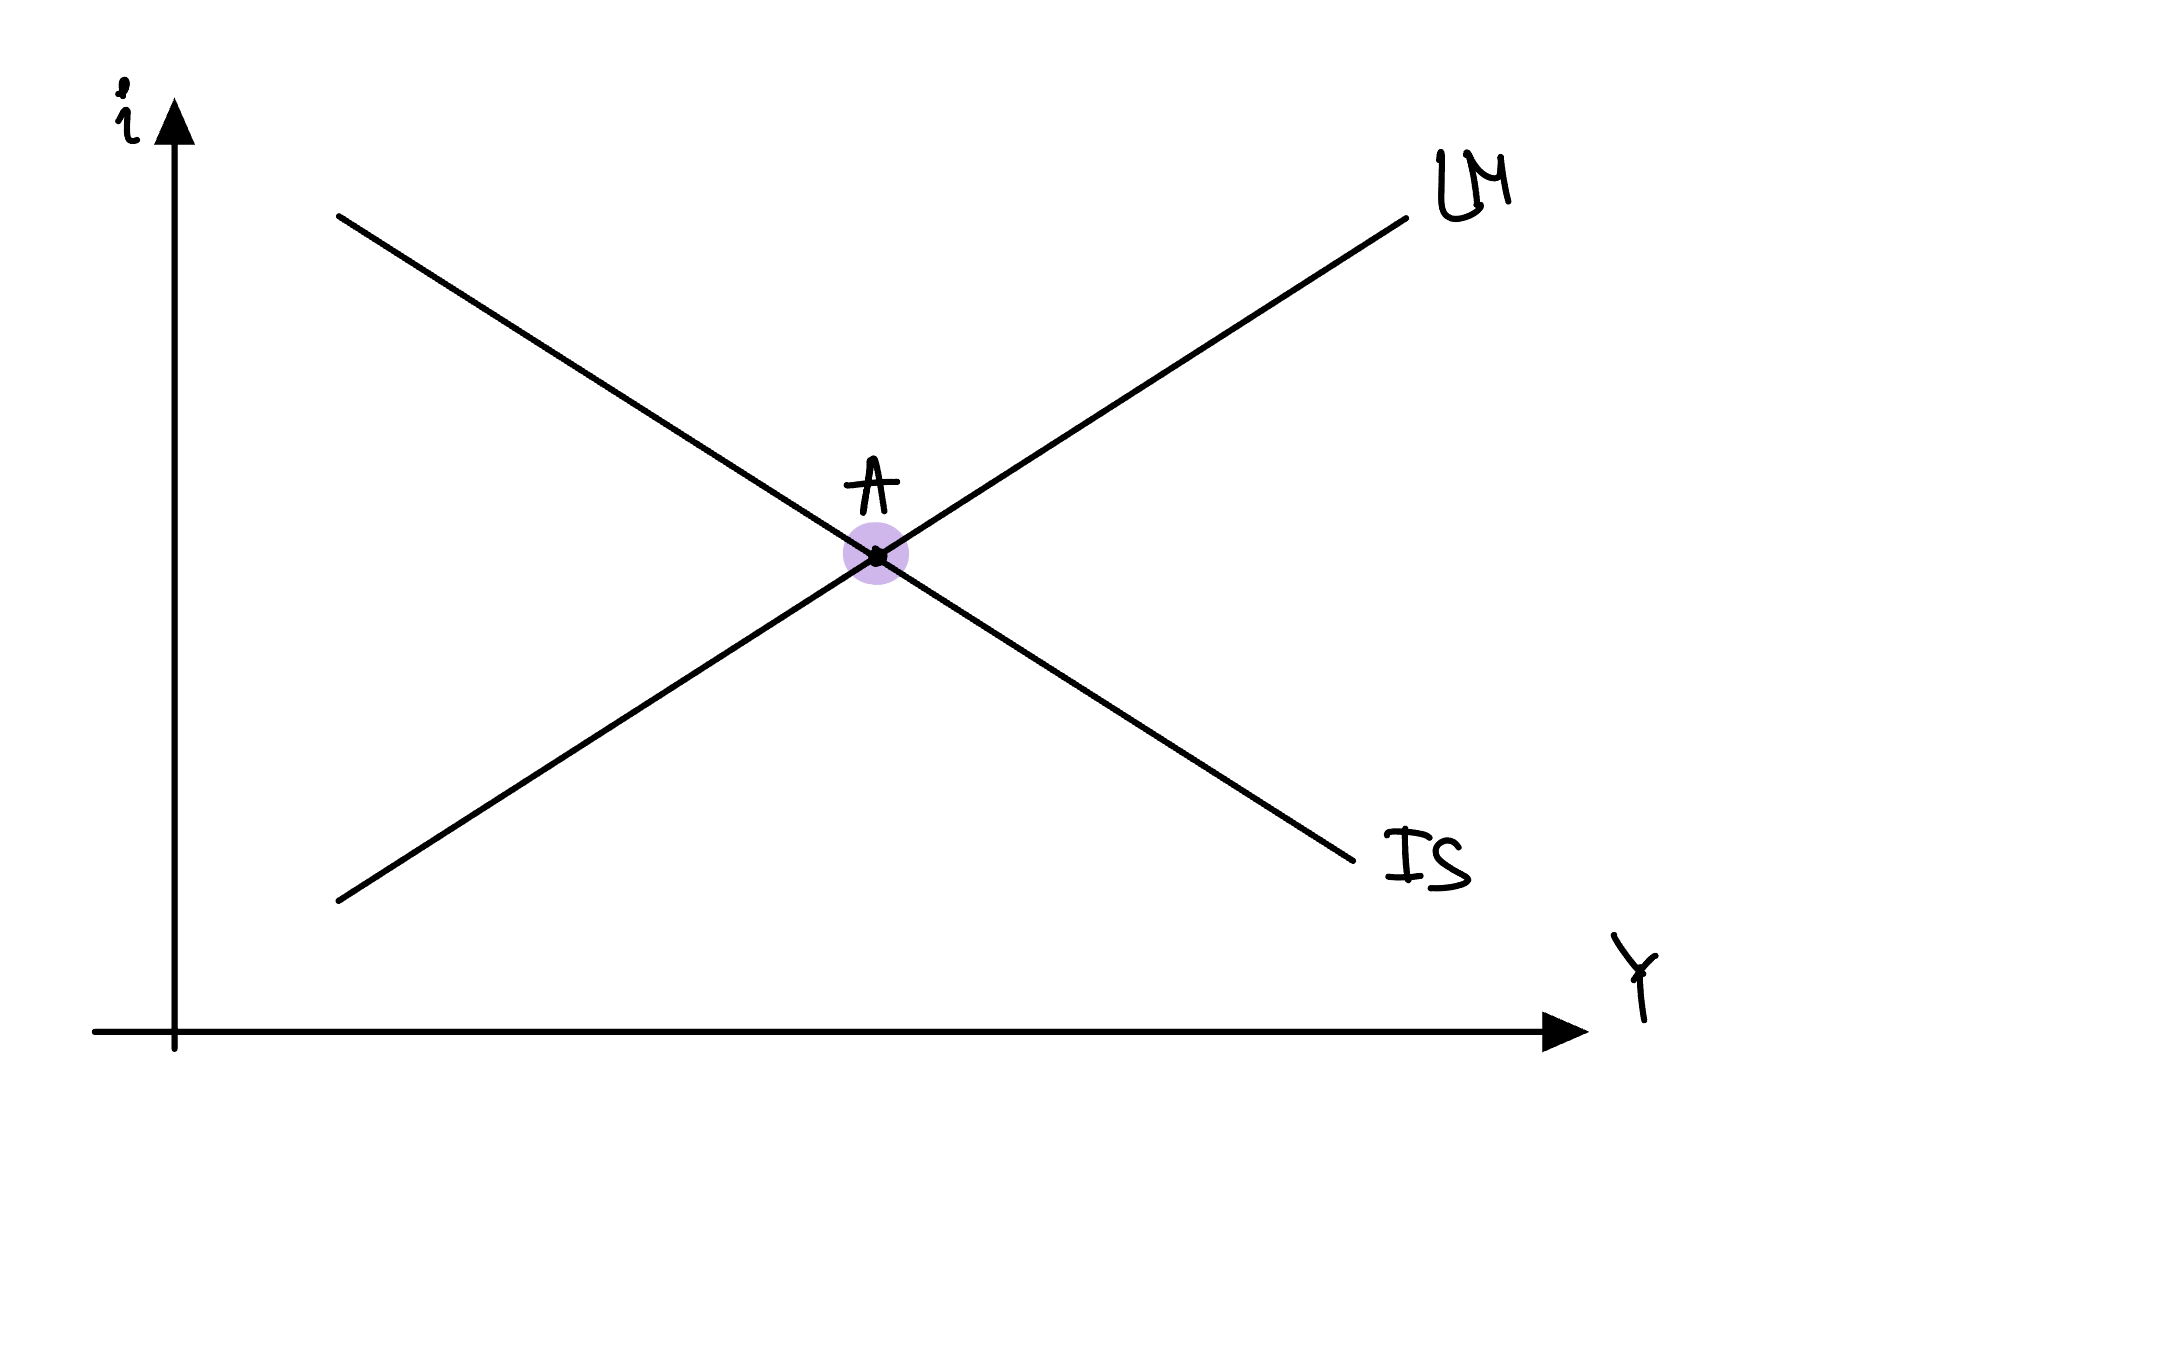
\includegraphics[width=0.95\textwidth]{figures/ISLM default.png}
        \end{center}
        % \caption{}
        \label{fig:}
    % \end{small}
\end{figure}

\begin{figure}[H]
    \begin{small}
        \begin{center}
            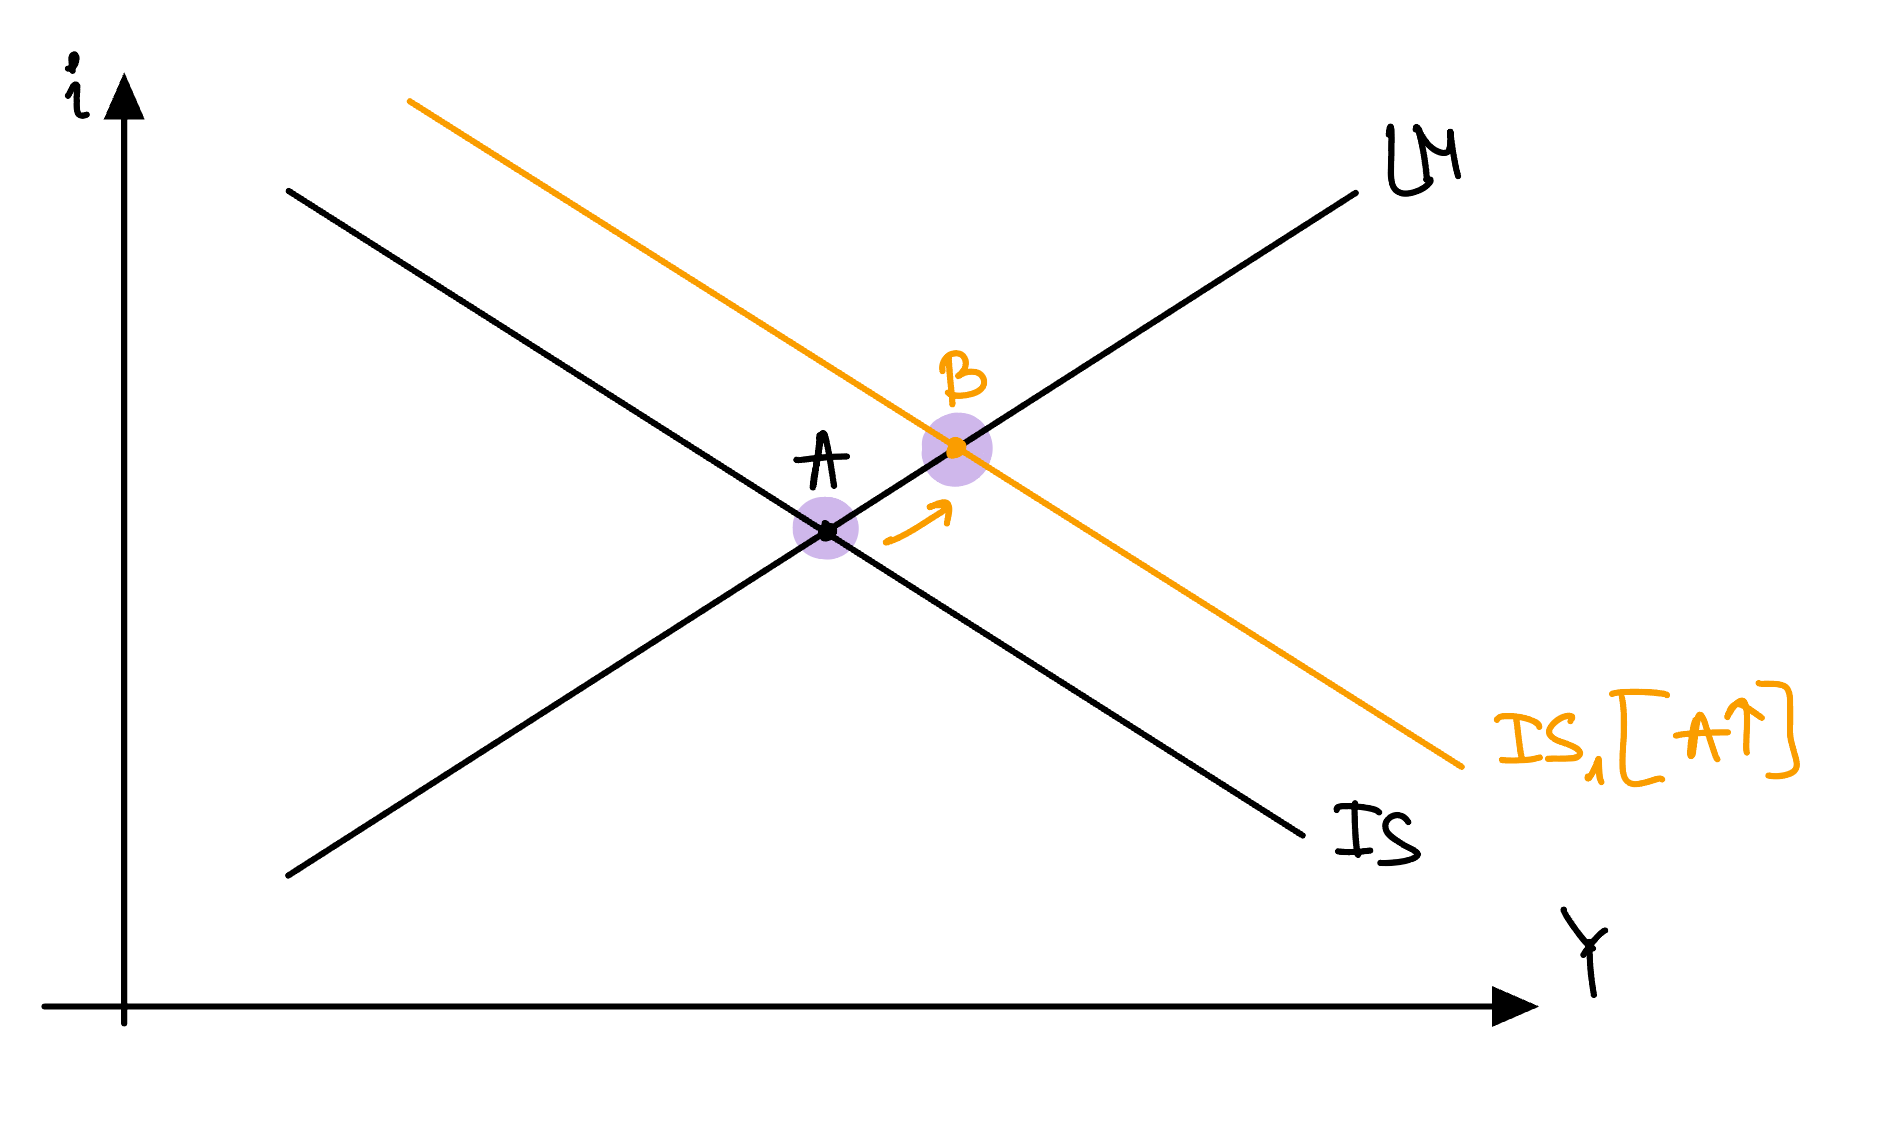
\includegraphics[width=0.95\textwidth]{figures/ISLM IS move.png}
        \end{center}
        % \caption{}
        \label{fig:}
    \end{small}
\end{figure}

\begin{figure}[H]
    \begin{small}
        \begin{center}
            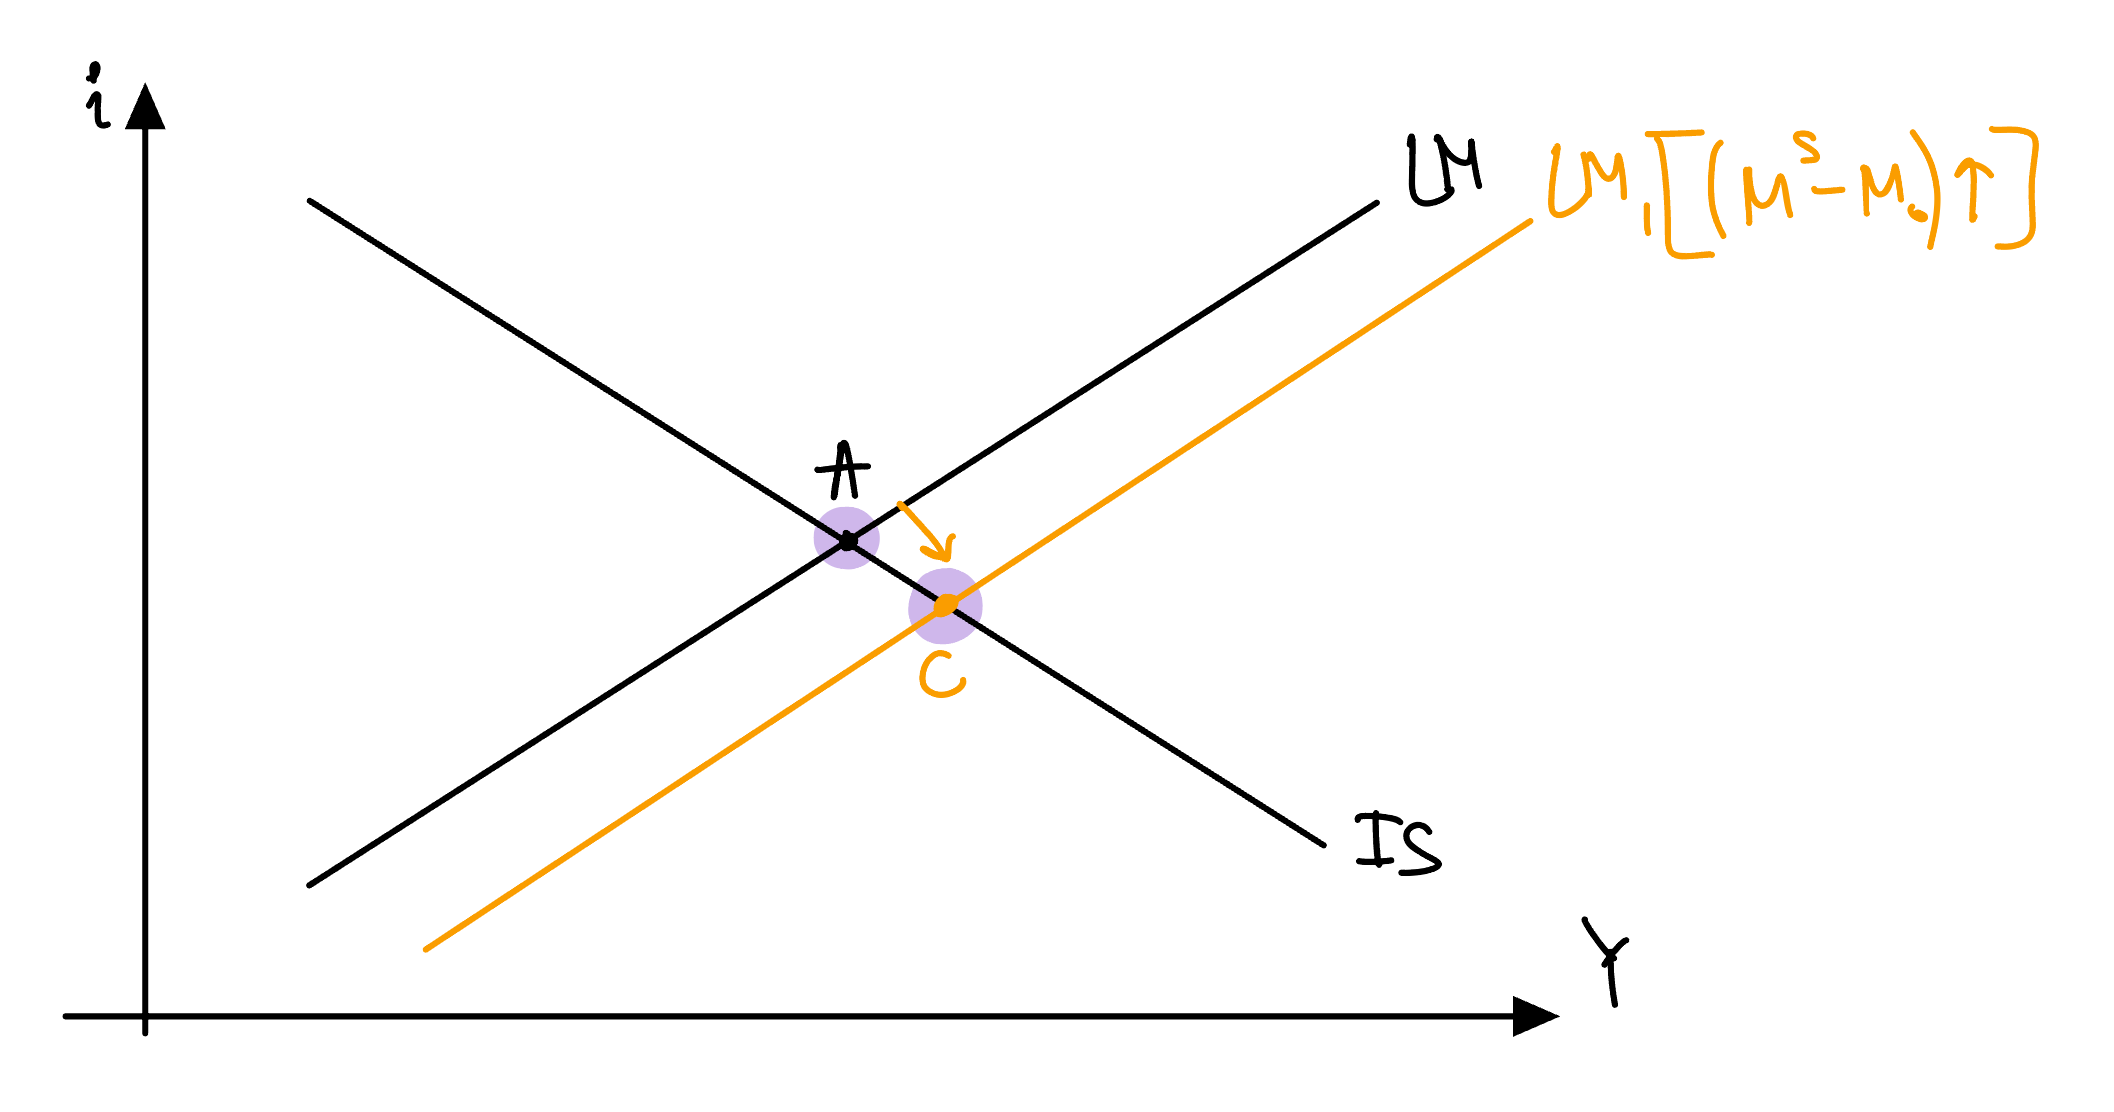
\includegraphics[width=0.95\textwidth]{figures/ISLM LM Move.png}
        \end{center}
        % \caption{}
        \label{fig:}
    \end{small}
\end{figure}




\end{RTL}
\end{document}